\documentclass[12pt]{ctexart}
\CTEXsetup[format={\Large\bfseries}]{section}
\usepackage{graphicx}
\usepackage{geometry}
\usepackage{fancyhdr}
\pagestyle{fancy}                                              
\fancyhead{} %clear all fields                                 
\pagestyle{empty}
\usepackage{amsmath}
\usepackage{amsfonts}
\usepackage{amssymb}
\usepackage{color}
\usepackage{multirow}
\usepackage{extarrows}
\usepackage{float}
\usepackage{makecell,multirow,diagbox}
\makeatletter  
\newif\if@restonecol  
\makeatother  
\let\algorithm\relax  
\let\endalgorithm\relax  
\usepackage[linesnumbered,ruled,vlined]{algorithm2e}{  
\usepackage{algpseudocode}  
\usepackage{amsmath}  
\renewcommand{\algorithmicrequire}{\textbf{Input:}}  % Use Input in the format of Algorithm  
\renewcommand{\algorithmicensure}{\textbf{Output:}} % Use Output in the format of Algorithm   
\geometry{left = 1cm, right = 1cm, top = 1.0cm, bottom = 1.8cm}
\newcommand{\eqdef}{\xlongequal{\text{def}}}%
\begin{document}
	
\author{敖睿成}
\title{应用数学导论大作业}\date{}
\maketitle

\section{摘要}
考虑方程
$$\left\{
\begin{aligned}
&\frac{\partial u}{\partial t} = \Delta u\\
&\mbox{边值条件} \\
\end{aligned}
\right.$$
本次实验中,依次针对一维情形,$ \Omega = [0,1]\times [0,1]$,L-型区域上的泊松问题,分别使用有限元方法,和中心差分方法求解方程,并给出相关理论分析和实验结果。

\section{一维自适应有限元方法}
对一维问题
$$\left\{
\begin{aligned}
&-u'' = f\indent \Omega = (0,L) \\
& u'(0) =\kappa_0(u(0)-g_0) \\
& u'(L) = \kappa_L(u(L)-g_L)\\
\end{aligned}
\right.$$
对于$N+1$个结点$x_0=0,x_1 = \frac{L}{N},...x_N=L,$在子区间$[x_{i-1},x_{i+1}](i=1,2,...,N-1)$上取分段线性函数:
$$\phi_i(x)=\left\{
\begin{aligned}
&\frac{x-x_{i-1}}{h_i},\indent x\in[x_{i-1},x_i]\\
&\frac{x_{i+1}-x}{h_{i+1}},\indent x\in [x_i,x_{i+1}] \\
&0,	\indent 其他
\end{aligned}
\right.$$其中$h_i=x_i-x_{i-1},$对于边界两个结点,考虑$x_0,x_1;x_{N-1},x_N$对应的两个两点线性插值函数,这样得到$N+1$个基函数$\phi_0,\phi_1,...,\phi_N,$现求解$v(x)= \sum_{j=0}^{N}u_j\phi_j(x)$,使得
$$ -\int_{0}^{1}u''(x)v(x)dx = \int_{0}^{1}f(x)v(x)dx $$
成立,通过变分方法得到:
$$\left\{
\begin{aligned}
 -\frac{u_{i-1}}{h_i}+(\frac{1}{h_i}+\frac{1}{h_{i+1}})u_i-\frac{u_{i+1}}{h_{i+1}} &= \int_{x_{i-1}}^{x_{i+1}}f\phi'(x)dx \indent i=1,2,...,N-1\\
(\frac{1}{h_1}+\kappa_0)u_0-\frac{u_1}{h_1} &= f_0 \\
(\frac{1}{h_N}+\kappa_L)u_N-\frac{u_{N-1}}{h_N} &= f_N \\
\end{aligned}
\right.
$$
令$a_i = \frac{1}{h_i}+\frac{1}{h_{i+1}},i=1,2,...,N-1,$
$$
A = 
\begin{pmatrix}
\frac{1}{h_1}+\kappa_0 & -\frac{1}{h_1}\\
-\frac{1}{h_1}& a_1& -\frac{1}{h_2} \\
& -\frac{1}{h_2}& a_2 & \ddots \\
& & \ddots & \ddots & -\frac{1}{h_{N}}\\
& & & -\frac{1}{h_{N}} & \frac{1}{h_N}+\kappa_L 
\end{pmatrix}
$$
得到方程$$Au = F$$。分别应用均匀剖分和自适应方法,在总点数$N=10,20,80$时得到如下结果:\\
$\kappa_0=10^6,k_1=0,g_0=0,f(x)=e^{-100(x-0.5)^2}$时,\\
\begin{figure}[H]
	\centering
	\begin{minipage}[t]{0.48\textwidth}
		\centering
		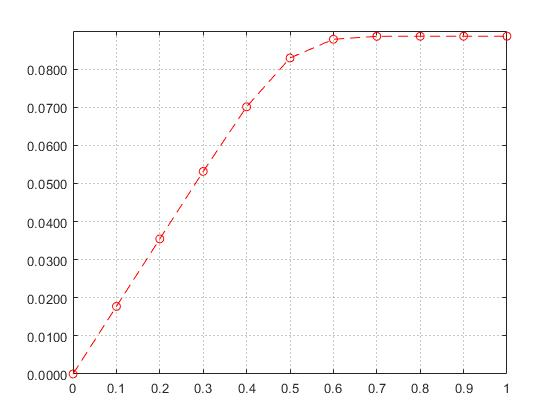
\includegraphics[width=9cm]{方程一,均匀剖分10.jpg}
		\caption{均匀剖分10}
	\end{minipage}
	\begin{minipage}[t]{0.48\textwidth}
		\centering
		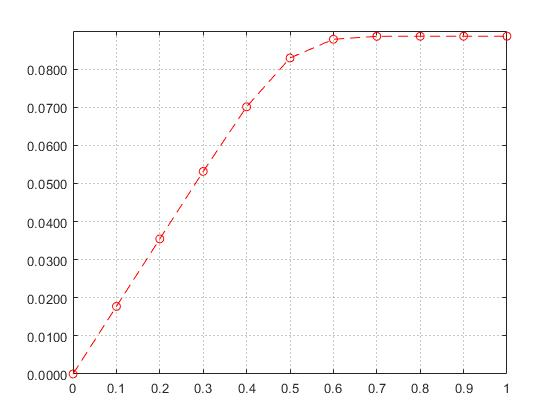
\includegraphics[width=9cm]{方程一,自适应10.jpg}
		\caption{自适应10}
	\end{minipage}
\end{figure}
\begin{figure}[H]
	\centering
	\begin{minipage}[t]{0.48\textwidth}
		\centering
		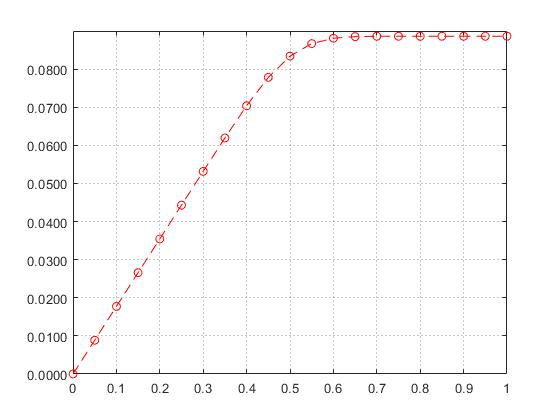
\includegraphics[width=9cm]{方程一,均匀剖分20.jpg}
		\caption{均匀剖分20}
	\end{minipage}
	\begin{minipage}[t]{0.48\textwidth}
		\centering
		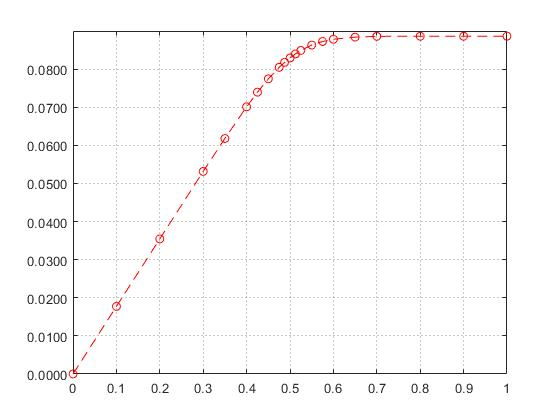
\includegraphics[width=9cm]{方程一,自适应20.jpg}
		\caption{自适应20}
	\end{minipage}
\end{figure}
\begin{figure}[H]
	\centering
	\begin{minipage}[t]{0.48\textwidth}
		\centering
		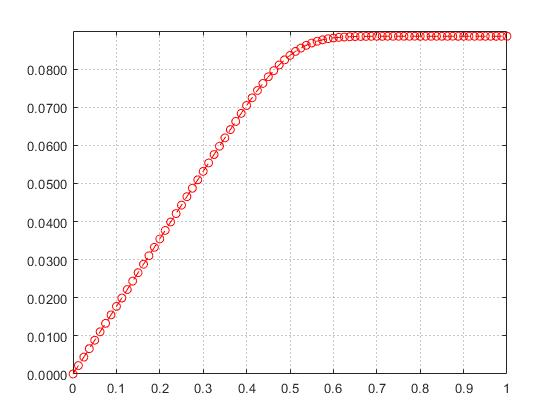
\includegraphics[width=9cm]{方程一,均匀剖分80.jpg}
		\caption{均匀剖分80}
	\end{minipage}
	\begin{minipage}[t]{0.48\textwidth}
		\centering
		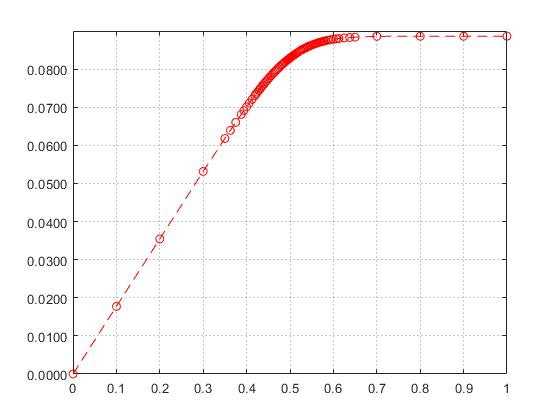
\includegraphics[width=9cm]{方程一,自适应80.jpg}
		\caption{自适应80}
	\end{minipage}
\end{figure}
$\kappa_0=10^6,k_1=10^5,g_0=0,g_L=0,f(x)=e^{-100(x-0.5)^2}$时,\\
\begin{figure}[H]
	\centering
	\begin{minipage}[t]{0.48\textwidth}
		\centering
		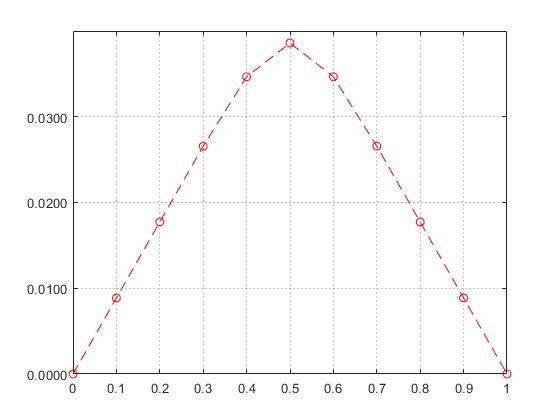
\includegraphics[width=9cm]{方程二,均匀剖分10.jpg}
		\caption{均匀剖分10}
	\end{minipage}
	\begin{minipage}[t]{0.48\textwidth}
		\centering
		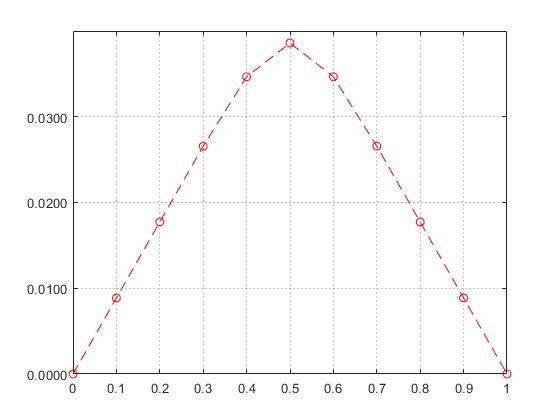
\includegraphics[width=9cm]{方程二,自适应10.jpg}
		\caption{自适应10}
	\end{minipage}
\end{figure}
\begin{figure}[H]
	\centering
	\begin{minipage}[t]{0.48\textwidth}
		\centering
		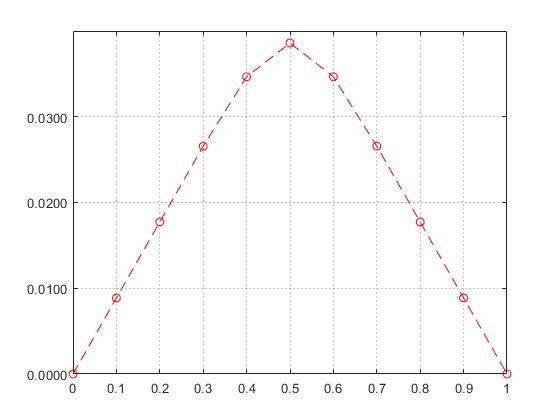
\includegraphics[width=9cm]{方程二,均匀剖分10.jpg}
		\caption{均匀剖分20}
	\end{minipage}
	\begin{minipage}[t]{0.48\textwidth}
		\centering
		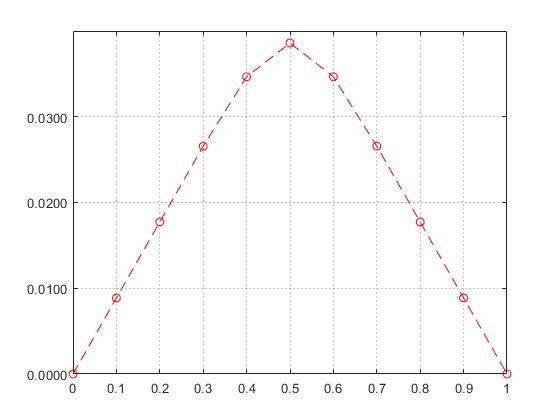
\includegraphics[width=9cm]{方程二,自适应10.jpg}
		\caption{自适应20}
	\end{minipage}
\end{figure}
\begin{figure}[H]
	\centering
	\begin{minipage}[t]{0.48\textwidth}
		\centering
		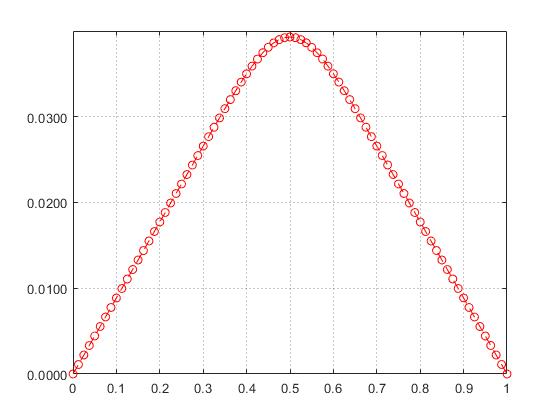
\includegraphics[width=9cm]{方程二,均匀剖分80.jpg}
		\caption{均匀剖分80}
	\end{minipage}
	\begin{minipage}[t]{0.48\textwidth}
		\centering
		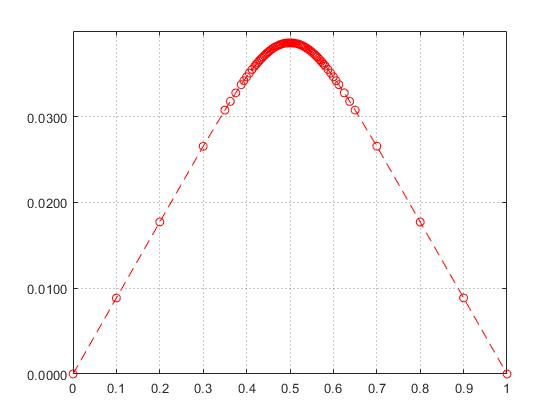
\includegraphics[width=9cm]{方程二,自适应80.jpg}
		\caption{自适应80}
	\end{minipage}
\end{figure}
$\kappa_0=10^6,k_1=0,g_0=-1,f(x)=e^{-100(x-0.5)^2}$时,\\
\begin{figure}[H]
	\centering
	\begin{minipage}[t]{0.48\textwidth}
		\centering
		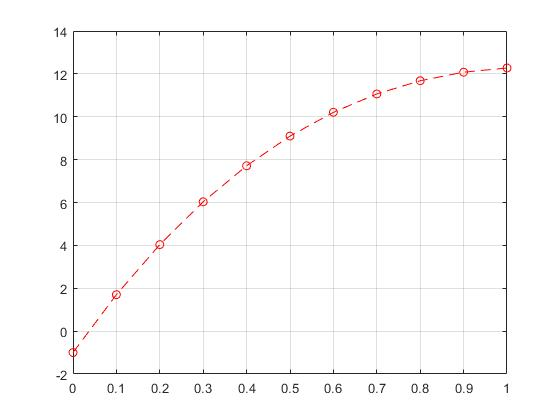
\includegraphics[width=9cm]{方程三,均匀剖分10.jpg}
		\caption{均匀剖分10}
	\end{minipage}
	\begin{minipage}[t]{0.48\textwidth}
		\centering
		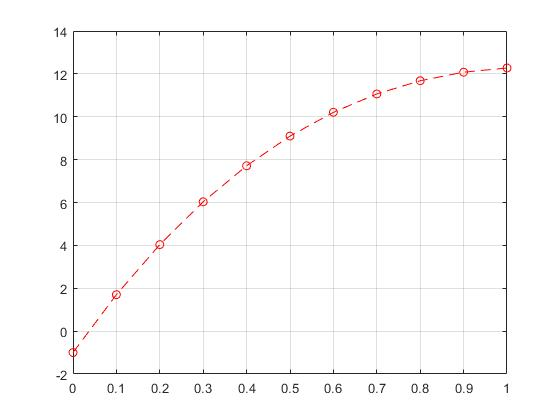
\includegraphics[width=9cm]{方程三,自适应10.jpg}
		\caption{自适应10}
	\end{minipage}
\end{figure}
\begin{figure}[H]
	\centering
	\begin{minipage}[t]{0.48\textwidth}
		\centering
		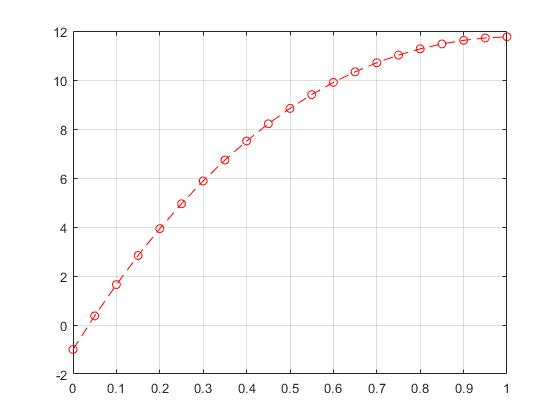
\includegraphics[width=9cm]{方程三,均匀剖分20.jpg}
		\caption{均匀剖分20}
	\end{minipage}
	\begin{minipage}[t]{0.48\textwidth}
		\centering
		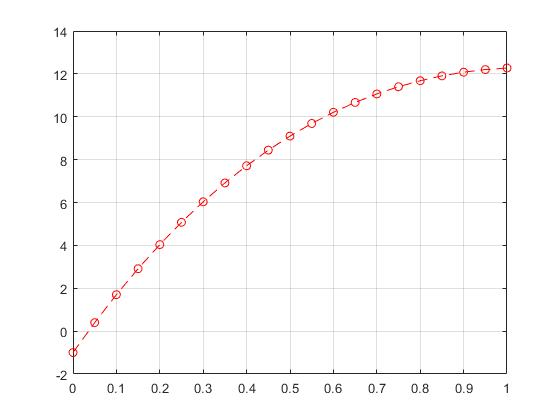
\includegraphics[width=9cm]{方程三,自适应20.jpg}
		\caption{自适应20}
	\end{minipage}
\end{figure}
\begin{figure}[H]
	\centering
	\begin{minipage}[t]{0.48\textwidth}
		\centering
		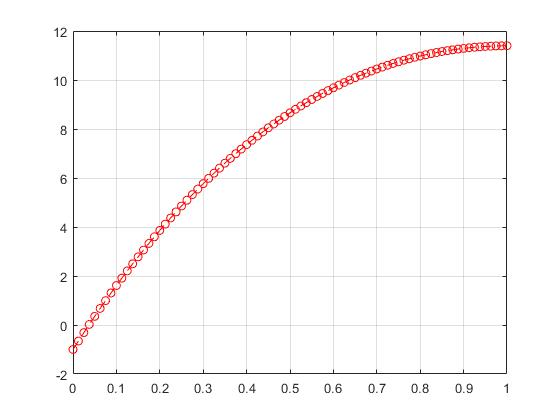
\includegraphics[width=9cm]{方程三,均匀剖分80.jpg}
		\caption{均匀剖分80}
	\end{minipage}
	\begin{minipage}[t]{0.48\textwidth}
		\centering
		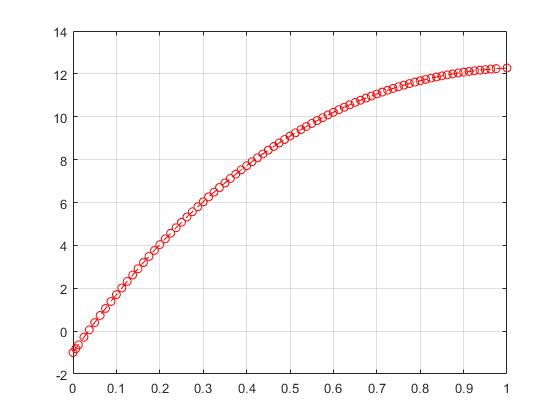
\includegraphics[width=9cm]{方程三,自适应80.jpg}
		\caption{自适应80}
	\end{minipage}
\end{figure}
可以看到,相比较均匀剖分,自适应方法在曲率大的点附近加密得较细,所得函数也更为平滑。
\section{正方形区域泊松方程}
\subsection{问题}
考虑热传导方程:
$$
\left\{
\begin{aligned}
&\frac{\partial u}{\partial t} = \Delta u\\
&u|_{\partial \Omega\times[0,1]} = 0, \Omega = [0,1]\times [0,1]\\
&u|_{t=0}=\sin(\pi x)\sin(\pi y)
\end{aligned}
\right.
$$
它有解析解$u = e^{-2\pi^2t}\sin(\pi x)\sin(\pi y)$,我们使用不同数值方法计算方程近似解,并给出相关分析。
\subsection{稳定性分析}
考察Laplace算子$$\Delta = \frac{\partial^2}{\partial x^2} + \frac{\partial^2}{\partial y^2}$$
\noindent 我们使用中心差分方法
$$
L_{h_x,h_y}U_{i,j}^m \eqdef \frac{U_{i-1,j}^m-2U_{i,j}^m+U_{i+1,j}^m}{h_x^2} + \frac{U_{i,j-1}^m-2U_{i,j}^m+U_{i,j+1}^m}{h_y^2}
$$
\noindent
这里$h_x,h_y$为对应分量的区间步长,对于$\frac{\partial u}{\partial t}$,\noindent 我们使用一阶向前差分方法:
$$
D_k U_{i,j}^m \eqdef \frac{U_{i,j}^{m+1}-U_{i,j}^m}{k}
$$
这里$k$为时间步长。现在考虑等式:
$$
(1-\theta)L_{h_x,h_y}U_{i,j}^m+\theta L_{h_x,h_y}U_{i,j}^{m+1} = D_kU_{i,j}^m
$$
当$\theta = 1$时,为隐式格式,$\theta=0.5$时,为Crank-Nicolson格式,$\theta=0$时,为显式格式。令
$$\tilde{U} = u\left(ih_x,jh_y,\left(m+\frac{1}{2}\right)k\right)$$
应用Taylor公式,可以得到
$$
\begin{aligned}
L_{hx,hy}U_{i,j}^m =& \tilde{U}_{xx} + \tilde{U}_{yy} + \frac{2}{3!}\left(3\tilde{U}_{txx}\left(-\frac{1}{2}k\right)+3\tilde{U}_{tyy}\left(-\frac{1}{2}k\right)\right) \\
&+\frac{2}{4!}\left(\tilde{U}_{xxxx}h_x^2+\tilde{U}_{yyyy}h_y^2\right)+O(k^2+h_x^4+h_y^4)
\end{aligned}
$$
$$
\begin{aligned}
L_{hx,hy}U_{i,j}^{m+1} =& \tilde{U}_{xx} + \tilde{U}_{yy} + \frac{2}{3!}\left(3\tilde{U}_{txx}\frac{1}{2}k+3\tilde{U}_{tyy}\frac{1}{2}k\right) \\
&+\frac{2}{4!}\left(\tilde{U}_{xxxx}h_x^2+\tilde{U}_{yyyy}h_y^2\right)+O(k^2+h_x^4+h_y^4)
\end{aligned}
$$
从而有:
$$
\begin{aligned}
(1-\theta)L_{h_x,h_y}U_{i,j}^m+\theta L_{h_x,h_y}U_{i,j}^{m+1} - \Delta \tilde{U} =& \left(\left(\theta - \frac{1}{2}\right)k+\frac{h_x^2}{12}\right)\tilde{U}_{xxxx}+\left(\left(\theta - \frac{1}{2}\right)k+\frac{h_y^2}{12}\right)\tilde{U}_{yyyy}\\
&+\left(2\theta - 1\right)k\tilde{U}_{xxyy} + O(k^2+h_x^4+h_y^4)
\end{aligned}
$$
从而
$$
\begin{aligned}
(1-\theta)L_{h_x,h_y}U_{i,j}^m+\theta L_{h_x,h_y}U_{i,j}^{m+1} - \Delta \tilde{U} =& \left(\left(\theta - \frac{1}{2}\right)k+\frac{h_x^2}{12}\right)\tilde{U}_{xxxx}+\left(\left(\theta - \frac{1}{2}\right)k+\frac{h_y^2}{12}\right)\tilde{U}_{yyyy}\\
&+\left(2\theta - 1\right)k\tilde{U}_{xxyy} + O(k^2+h_x^4+h_y^4)
\end{aligned}
$$
这样截断误差$E$满足
$$
E = 
\begin{cases}
O(k^2+h_x^2+h_y^2) & \theta = 0.5\\
O(k+h_x^2+h_y^2) & \theta \neq 0.5\\
O(k+h_x^4+h_y^4) & h_x = h_y,\theta = 0.5-1/12\mu_x \\
\end{cases}
$$
可以看出,C-N方法具有较高的截断误差阶数,现在考虑Fourier函数
$$U_{j,k}^m =\lambda_{\alpha}^me^{i(\alpha_xx_j+\alpha_yy_k)},\quad \alpha = (\alpha_x, \alpha_y)$$
解得
$$
\lambda_k = \frac{1 - 4(1-\theta)\left(\mu_x\sin^2(\alpha_xh_x/2)+\mu_y\sin^2(\alpha_yh_y/2)\right)}{1+4\theta\left(\mu_x\sin^2(\alpha_xh_x/2)+\mu_y\sin^2(\alpha_yh_y/2)\right)}
$$
因此,我们有稳定性条件

$$
\left\{
\begin{aligned}
	2(\mu_x+\mu_y)(1-2\theta) \le 1  \indent&0 \le \theta < 1/2\\
	\mbox{无条件收敛} \indent \indent  &1/2 \le \theta \le 1
\end{aligned}
\right.
$$
这表明当$h_x = h_y =h$时,对于显式格式,我们需要选取$\mu < \frac{1}{4}$,即$1/h \ge 1/4k$,才能得到收敛结果。
\subsection{数值实验}
考虑由中间$(N-1)\times(N-1)$个点,其中$N=\frac{1}{h}$为单元网格长,则对应的差分矩阵
$$
\L_h = 
\begin{pmatrix}
A_h & I_{N-1}/h\\
I_{N-1}/h^2 & A_h & I_{N-1}/h^2 \\
& I_{N-1}/h^2 & A_h & \ddots \\
& & \ddots & \ddots & I_{N-1}/h^2\\
& & & I_{N-1}/h^2 & A_h
\end{pmatrix}
$$
$$
A_h = 
\begin{pmatrix}
-2/h^2-2/h^2 & 1/h^2\\
1/h^2 & -2/h^2-2/h^2 & 1/h^2 \\
& 1/h^2 & -2/h^2-2/h^2 & \ddots \\
& & \ddots & \ddots & 1/h^2\\
& & & 1/h^2 & -2/h^2-2/h^2
\end{pmatrix}
$$
这样,得到如下方程
$$
(I - k\theta L_h)U^{m+1} = (I + k(1 - \theta)L_h)U^m
$$
其中$U$为对应的网格向量化。下面考虑几种求解对应方程的方法。\\
\noindent \textbf{Cholesky分解}\\
考察方程$Ax=b$,其中A为对称正定矩阵,则我们有如下Cholesky分解用以求解方程:\\
\begin{algorithm}[H]
	\caption{利用向量外积的cholesky分解}  
	\label{alg:gaxpy chol}
	\KwIn{$A \in \mathbb{R}^{n\times n}$}  
	\KwOut{$L \in \mathbb{R}^{n\times n}$,\ $LL^{\rm T} = A$}  
	\For{$j=1 : n$}  
	{ 
		\If{$j > 1$}
		{
			$A(j:n,j) = A(j:n,j) - A(j:n,1:j-1)A(j,1:j-1)^{\rm T}$
		}
		$A(j:n,j) = A(j:n,j)/\sqrt{A(j,j)}$		
	}  
	\Return $tril(A)$\;
\end{algorithm}
\noindent 计算量约为$O(n^3/3)$,是直接进行Gauss消元法的一半,在矩阵阶数较小时具有很快速度,但当矩阵阶数较大时,可以使用分块的方法加快速度。\\
\noindent \textbf{Gauss-Seidel迭代法}\\
令$A = D-L-U$,其中$D,L,U$分别为对角矩阵、下三角矩阵和上三角矩阵,则我们有如下算法:\\
\begin{algorithm}[H]
	\caption{G-S迭代法}  
	\label{alg:GS}
	\KwIn{$A \in \mathbb{R}^{n\times n}$,$b \in \mathbb{R}^n$, \textbf{TOLERENCE} $tol$, \textbf{INITIALVALUE} $x_0$ \textbf{MAXITERATION} $ite$}
	\KwOut{$x \in \mathbb{R}^{n}$,\ $Ax \approx b$}
	Divide $A$ into $D$,$L$ and $U$\\
	$\mathbf{Ux} \gets Ux_0$\\
	\While{$norm(res)/norm(res_0) > tol \indent\textbf{\&\&} ite_number\le ite  $}
		{
			Get $x$ by solving $(D-L)x = \mathbf{Ux} + b$\\
			Update $res = Ux - \mathbf{Ux}$\\
			Update $\mathbf{Ux} \gets res + \mathbf{Ux}$\\
			\If{\text{norm}($res$) $\le tol*res_0$}{
				\Return $x$\\
		}
	}
	\Return $x$\;
\end{algorithm}
\noindent 这里利用到了$\text{res} = b - Ax^{m+1} = b - (D-L)x^{m+1} + Ux^{m+1} = Ux^{m+1} - Ux^m$。可以证明,当A为对称正定矩阵时,G-S迭代法是收敛的。\\
\noindent \textbf{多重网格法}\\
对于单元格长为$h=1/N$的细网格,我们希望找到一个较好的初始值,从而加快迭代法收敛的速度,故考虑在细网格上先进行若干次迭代,再将误差限制在粗网格上,在粗网格解关于误差的方程,再把提升回细网格,这样两者相加,可以认为得到了更近的初值,再重复这样的操作,直到误差满足要求,这里可以重复限制、提升多层,算法如下:\\
\begin{algorithm}[H]
	\caption{多重网格法}
	\label{alg:MG}  
	\KwIn{$A \in \mathbb{R}^{n\times n}$,$b \in \mathbb{R}^n$, \textbf{EDGE} $h$, \textbf{MAXITERATION} ${ite}_1$, \textbf{INITIALVALUE} $x_0$}
	\KwOut{$x \in \mathbb{R}^{n}$,\ $Ax \approx b$}
	\If{$size(x) < threshold$}{
		Solve $Ax = b$ by \textbf{G-S} with \textbf{INITIALVALUE} $x_0$\\
	}
	\Else{
		Solve $Au = b$ by \textbf{G-S} with \textbf{INITIALVALUE} $x_0$ and \textbf{MAXITERATION} ${ite}_1$\\
		Get residue: $res \gets b - Au$\\
		Get coarse residue: $\widehat{res} \gets I_{h}^{2h}res$\\
		$\widehat{A} \gets I_{h}^{2h}A\:I_{2h}^h$\\
		Solve $\widehat{A}\hat{e} = \widehat{res}$ with \textbf{EDGE} $2*h$, \textbf{INITIALVALUE} $0$ and \textbf{MAXITERATION} $ite$ by \textbf{G-S} \\
		$e \gets I_{2h}^h\hat{e}$\\
		Update $u \gets u + e$\\
		Solve $Ax = b$ by \textbf{G-S} with \textbf{INITIALVALUE} $u$ and \textbf{MAXITERATION} ${ite}_2$\\
	}
	\Return $x$\;
\end{algorithm}
\noindent 这里$I_{h}^{2h},I_{2h}^{h}$分别为限制和提升矩阵。当初始值较差时,多重网格的速度一般比直接G-S迭代快。\\
\noindent \textbf{数值结果}\\
对于近似解$\tilde{U}_{h}$,在每个单元上使用双线性函数来逼近原区域。对于单元K,定义映射:
$$\tilde{F}:\xi=\frac{2(x-x_c)}{h_x},\eta=\frac{2(y-y_c)}{h_y},\indent (x,y)\in K,(\xi,\eta)\in \tilde{K}$$
定义如下的基函数:
$$
	\begin{aligned}
& \Phi_1 = \frac{(1-\xi)(1-\eta)}{4},\Phi_2=\frac{(1-\xi)(1-\eta)}{4}\\
& \Phi_3 = \frac{(1+\xi)(1-\eta)}{4},\Phi_4=\frac{(1+\xi)(1+\eta)}{4}\\
\end{aligned} 
$$
令$u_h(x,y)|_{K}=\hat{u}(\xi,\eta)=\sum_{i=1}^{4}u_i\Phi_i(\xi,\eta)$,我们计算误差
$$||u(x,y,1)-u_{h}(x,y,1)||_0= (\int_{\Omega}(u(x,y,1)-u_h(x,y,1))^2dxdy)^{1/2}$$
和相对误差$$||u(x,y,1)-u_{h}(x,y,1)||_0/|\int_{\Omega}udxdy|$$
数值结果如下:\\
\begin{table}[H]
	\centerline{
		\begin{tabular}{|c|c|c|ccc|}
			\hline
			\multirow{2}*{空间步长 $h$} &\multirow{2}*{时间步长 $k$}&\multirow{2}*{$\mu$}& \multicolumn{3}{c|}{相对误差}\\
			\cline{4-6}
			& & & 显式格式 & 隐式格式 & Crank-Nicolson 格式\\
			\hline
			\multirow{5}*{1/64} & 1/256  & 16 & $+\infty$ & 2.6179 & 4.5217e-2  \\
			\cline{2-6}
			& 1/512  & 8 & $+\infty$ & 0.9135 & 7.5452e-3 \\
			\cline{2-6}
			& 1/2048  & 2 & $+\infty$ & 0.2629& 5.3124e-3  \\
			\cline{2-6}
			& 1/4096  & 1 & $+\infty$ & 7.6829e-2 & 5.2517e-3 \\
			\cline{2-6}
			& 1/16384 & 1/4 & 3.1562e-2 & 3.2415e-2 & 5.4135e-3 \\
			\hline
			\multirow{4}*{1/128} & 1/1024  & 16 & $+\infty$ & 5.3681 & 5.3267e-3  \\
			\cline{2-6}
			& 1/4096 & 4 & $+\infty$ & 0.4581 & 3.6782e-3 \\
			\cline{2-6}
			& 1/16384  & 1 & $+\infty$ &7.6582e-2 & 2.5791e-3  \\
			\cline{2-6}
			& 1/65536  & 1/4 & 8.3725e-3 & 8.2373e-3 & 4.7592e-3  \\
			\cline{2-6}
			\hline 
	\end{tabular}}
	\caption{不同离散格式在最终时间层$t=1$的稳定性比较}
	\label{table:稳定性}
\end{table}
\begin{figure}[H]
	\centering
	\begin{minipage}[t]{0.48\textwidth}
		\centering
		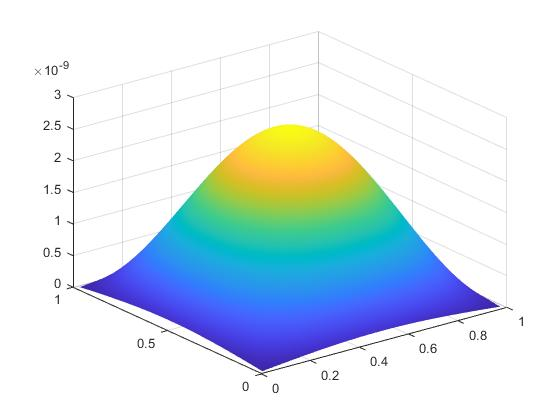
\includegraphics[width=9cm]{热扩散.jpg}
		\caption{$t=1$时图像}
	\end{minipage}
	\begin{minipage}[t]{0.48\textwidth}
		\centering
		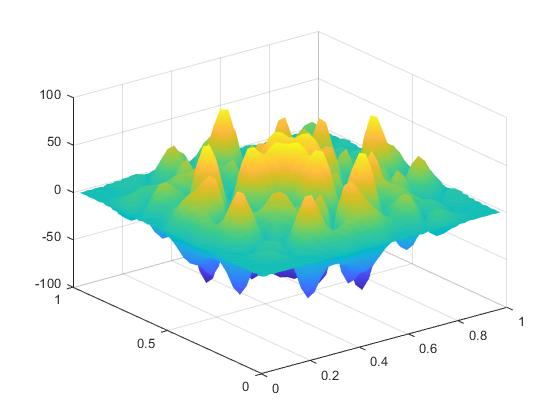
\includegraphics[width=9cm]{显式不稳定.jpg}
		\caption{$\mu>1/4$时显式格式}
	\end{minipage}
\end{figure}

\noindent 可以看到,与理论分析相同,当网格比$\mu > \frac{1}{4}$时,显式格式是不稳定的,而C-N方法在网格比较大时就有很好的稳定性,但随着网格比的减小和步长的减小,由于解方程的舍入误差,三者的表现最终接近,但步长很小时存在误差反而增大的情况,推测可能是由于方程的解析解较小,由于迭代造成的舍入损失更明显。\\
\indent 考虑取$h = 1/32,1/128,1/512,k = 1/512$,分别应用Chelesky分解,G-S迭代法和V-cycle多重网格法求解$t=1$的解,对于迭代法,每次以上一个时间层为初始值,所得时间分别如下:\\

\begin{table}[H]
	\centerline{
		\begin{tabular}{|c|c|c|c|c|}
			\hline
			\multirow{2}*{时间步长 $k$}& \multirow{2}*{空间步长 $h$} & \multicolumn{3}{c|}{总时间(s))}\\
			\cline{3-5}
			& & 多重网格 V& Cholesky & Gauss-Seidel\\
			\hline
			\multirow{3}*{1/512} &   1/32  & 1.3298e+1 & 7.2836  & 7.068  \\
			\cline{2-5}
			&   1/128  & 3.6337e+2 & 2.791 &  159.715 \\
			\cline{2-5}
			&   1/512  &  & 6.3446e+3 &  7.555e+3  \\
			\hline
	\end{tabular}}
	\caption{时间步长k=1/512时,三种方法求方程在$t=1$解的总时间}
	\label{table:CPU time}
\end{table}
\noindent 可以看出多重网格的时间大致为$O(N^2)$,Cholesky的时间为$O(N^6)$,而G-S迭代法所需的时间要多得多。\\
\indent
对每个固定的$h$,分别用三种格式求近似解,对每一种格式,令$k$从大到小依次取2的幂,比较它们的误差,取出其中最小的,并且计算误差$$||u(x,y,1)-u_{h}(x,y,1)||_0$$所得结果如下:\\
\begin{figure}[H]
	\centering
	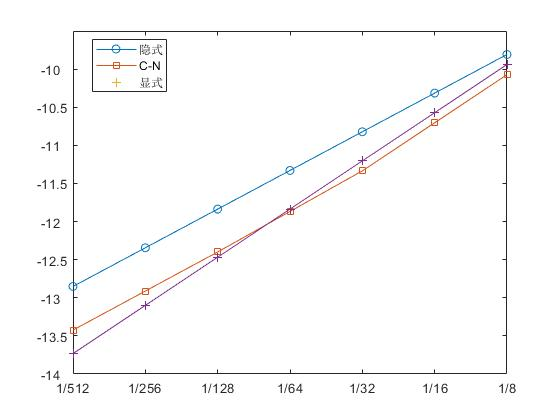
\includegraphics[width=12cm]{第三题图.jpg}
	\caption{对不同的$h$,选取最佳步长所得误差}
\end{figure}
\noindent 可以发现,虽然显式格式在$\lambda>1/4$时是发散的,但在适当的网格比下,反而可以得到很好的结果。
\section{L型区域上的泊松方程}
\subsection{问题}
考虑如下泊松问题:
$$
\begin{aligned}
-\Delta&=f\indent (x,y)\in \Omega,\\
u|_{\partial\Omega}&=0
\end{aligned}
$$
\noindent 其中区域$\Omega$为如下L型区域,$u(x,y)=r^{\frac{2}{3}}sin(\frac{2}{3}\theta)(1-x^2)(1-y^2)$。\\
\begin{figure}[H]
	\centering
	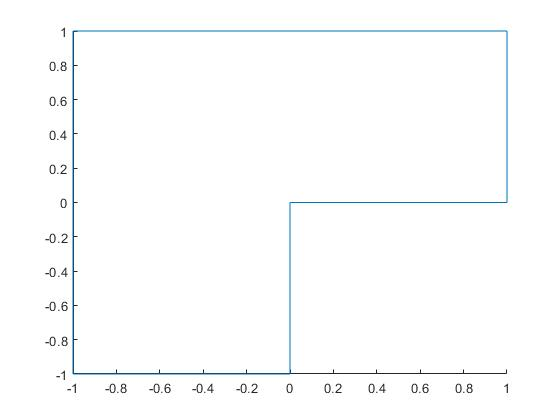
\includegraphics[width=12cm]{L-shaped.jpg}
	\caption{L型区域}
\end{figure}
\noindent 它的函数值和$\Delta$在$[0,1]\times[0,1]$区间上的图像如下:\\
\begin{figure}[H]
	\centering
	\begin{minipage}[t]{0.48\textwidth}
		\centering
		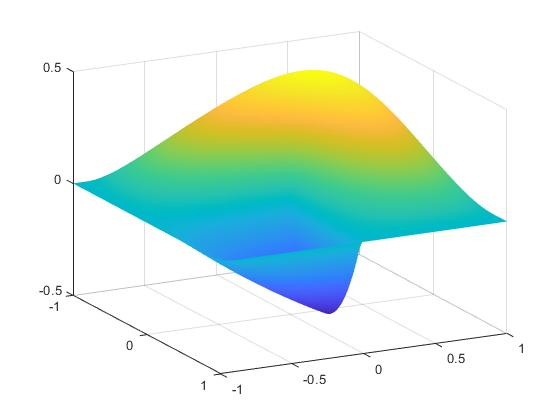
\includegraphics[width=9cm]{L-型函数.jpg}
		\caption{函数值}
	\end{minipage}
	\begin{minipage}[t]{0.48\textwidth}
		\centering
		\includegraphics[width=9cm]{L-型Laplace.jpg}
		\caption{$\Delta$}
	\end{minipage}
\end{figure}
\noindent 可以看到,在$(0,0)$的邻域内$\Delta\to +\infty$。下面我们分别使用均匀剖分和自适应剖分,利用差分方法求方程的近似解。
\subsection{数值实验}
\noindent \textbf{LDL分解}\\
考察方程$Ax=b$,对于对称非正定矩阵$A$,Cholesky分解不再有效,此时可以考虑同样利用了对称性的LDL分解,得到$A=LDL'$,依次求解$Lz=b,Dy=z,L'x=y$得到方程的解,这三个方程分别为下三角、对角、上三角的,可以在$O(n^2)$时间内求解,故LDL分解所需要的运算次数约为$O(n^3/3)$的,下面给出算法:\\
\begin{algorithm}[H]
	\caption{利用向量外积的LDL分解}  
	\label{alg:gaxpy ldl}
	\KwIn{$A \in \mathbb{R}^{n\times n}$}  
	\KwOut{$L,D \in \mathbb{R}^{n\times n}$, $LDL^{\rm T} = A$}  
	\For{$j=1 : n-1$}  
	{ 
		$A(j+1:n,j) = A(j+1:n,j)/A(j,j)$\\
		$A(j+1:n,j+1:n) = A(j+1:n,j+1:n)-A(j+1:n,j)*A(j,j+1:n)$\\	
	}  
	$L = tril(A,-1); D = diag(A)$\\
	\Return $L,D$\;
\end{algorithm}
当矩阵较大时,可以采用分块LDL分解,算法如下:\\
\begin{algorithm}[H]
	\caption{分块LDL分解}  
	\label{alg:chunk LDL}
	\KwIn{$A \in \mathbb{R}^{n\times n}$, \textbf{MINISIZE},\textbf{NUM}}  
	\KwOut{$L,D \in \mathbb{R}^{n\times n}$,\ $LDL^{\rm T} = A$}
	\If{$n \le  \textbf{MINISIZE}$}
	{
			Solve $A=LDL^{\rm T}$ with  \textbf{LDL分解}\\
	}  
	SUBSIDE = \textbf{CELL}(n/\textbf{NUM})
	\For{$j = 1 : SUBSIDE :n$}  
	{ 
		\If{$ j+$SUBSIDE$> n$}
		{
			Solve$ A(j:n,j:n) = LDL^{\rm T} $ with \textbf{LDL分解},update$ tril(A(j:n,j:n))\gets L,D$\\
		}
		\Else
		{
			Solve$ A(j:j+$SUBSIZE$-1,j:j+$SUBSIZE$-1)U'= A(j:j+$SUBSIZE$-1,j+SUBSIZE:n) $\\
			Update$A(j+$SUBSIZE$:n,j:j+$SUBSIZE$-1)\gets U $\\
			Update$A(j+$SUBSIZE$:n,j+$SUBSIZE$:n)\gets A(j+$SUBSIZE$:n,j+$SUBSIZE$:n)-A(j+$SUBSIZE$:n,j:j+$SUBSIZE$-1)*A(j:j+$SUBSIZE$-1,j+$SUBSIZE$:n)^{\rm T} $\\
			Solve$A(j:j+$SUBSIZE$-1,j:j+$SUBSIZE$-1) = LDL^{\rm T}$ with \textbf{分块LDL分解}\\
			Update$tril(A(j:j+$SUBSIZE$-1,j:j+$SUBSIZE$-1)) \gets L_1,D_1$\\
			Update$A(j+$SUBSIZE$:n,j+$SUBSIZE$:n)\gets L_1A(j+$SUBSIZE$:n,j+$SUBSIZE$:n)$\\
		}
		$L = tril(A,-1),D=diag(A)$\\
	}  
	\Return $L,D$\;
\end{algorithm}
\noindent \textbf{数值结果}\\
将L型区域分别以步长$h=h_x=h_y=2/N,N=32,64,128,256,512$进行均匀剖分,使用LDL分解,G-S迭代,松弛因子为1.5的超松弛迭代法,V-cycle多重网格法求解差分离散方程$A_hU_h=F_h$的解$U_h$或近似解$\tilde{U}_h$,其中系数矩阵为稀疏的对称正定矩阵,形如下图:\\
\begin{figure}[H]
	\centering
	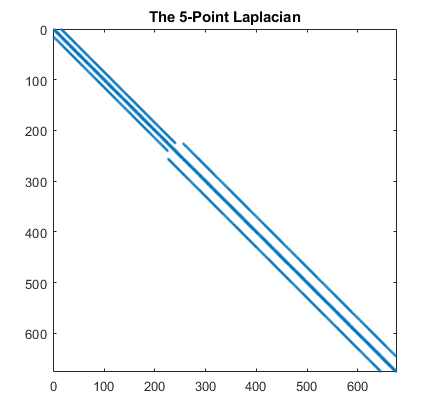
\includegraphics[width=12cm]{差分矩阵.png}
	\caption{L型差分系数矩阵}
\end{figure}
\noindent 其中编号的顺序是从右上角$(1-h,1-h)$开始,从上到下,从右往左编号。迭代法的初始值为全零网格,近似解$\tilde{U}_h$满足误差关系$$||A_h\tilde{U}_h-F_h||_2/||F_h||_2 \le 10^{-8} $$所花的时间如下:\\

\begin{table}[H]
	\centerline{
		\begin{tabular}{|c|c|c|c|c|}
			\hline
			\multirow{2}*{$N = 2/h$} &  \multicolumn{4}{c|}{总时间(s))}\\
			\cline{2-5}
		  	&LDL分解 & G-S迭代 V& 超松弛迭代 & 多重网格\\
			\hline
			32	&    9.1e-3  & 1.33e-2 & 8e-3  & 3.4e-3  \\
			\cline{1-5}
			64 & 5.11e-2 &   2.97e-1  & 7.67e-2 & 1.52e-2   \\
			\cline{1-5}
			128&   2.998e-1  & 6.1109 & 2.2015 & 6.62e-2   \\
			\cline{1-5}
			256& 2.5330 & 1.003e+2 & 3.6239e+1 &2.69e-1  \\
			\cline{1-5}
			512 &1.9108e+1 & 2.1589e+3 & 7.5086e+2 & 1.0992 \\
 			\hline
	\end{tabular}}
	\caption{时间步长k=1/512时,三种方法求方程在$t=1$解的总时间}
	\label{table:CPU time}
\end{table}
\noindent
接下来使用自适应剖分差分方法求解方程。格式如下:\\
\begin{algorithm}[H]
	\caption{L型区域自适应方法}  
	\label{alg:self adaptive}
	\KwIn{\textbf{INITIALGRID} $U_0$, \textbf{ERROR} $\varGamma_0$,$\theta$,\textbf{TOLERANCE} $\epsilon$,$k=0$}  
	\KwOut{$U,N$}  
	Update $\eta(\varGamma_{k-1})\gets \eta(\varGamma_{k}) $\\
	\While{\textbf{TRUE}}{
	\If{$\varGamma_{k}\le \epsilon$}
	{
		$N = k,U = U_k$ \textbf{Return} \\
	}
	Find minimal subset unit set $\mathcal{M}_k$ such that $\eta(\mathcal{M}_k)^2 \ge \theta\eta(\varGamma_k)^2$ \\
	Update $\varGamma_{k}\gets \varGamma_{k+1}$\\
	Update $k\gets k+1 $\\
	}
	\Return $N,U$\;
\end{algorithm}
\noindent
这里$\eta(\varGamma)$为后验误差估计因子:
$$
\eta_K^2 = h_K^2||f||_{L^2(K)}^2+\sum_{e\in\mathcal{E}_K}h_e||[\frac{\partial u_h}{\partial  n_e}]||_{L^2(e)'}^2	
$$
其中$h_K$是单元$K$最长边的长度,$\mathcal{E}$是$K$所有不在边界的边的集合,$h_e$是边$e$的长度,$n_e$是$e$上的外法向方向,$[\frac{\partial u_h}{\partial  n_e}]$是法向导数跨过$e$的跳跃,即
$$
\frac{\partial u_h}{\partial  n_e}|_{K^+}-\frac{\partial u_h}{\partial  n_e}|_{K^-}
$$
$\eta(G)$表示单元集合$G$中所有单元的后验误差之和。每次剖分把所选集合中的单元加细,并将边界上有两个悬点的单元也加细,使得任意一个单元的边界上只有至多一个悬点。需要注意的是,在计算中悬点取边两端点函数值的均值。分别以$\theta=0.8,0.6,0.3,0.2,0.1,\epsilon=10^{-6}$,一般来说,$\theta$越大,每次加密得网格越多,单步时间越长,收敛的步数越少。得出网格剖分图如下:\\
\begin{figure}[H]
	\centering
	\begin{minipage}[t]{0.48\textwidth}
		\centering
		\includegraphics[width=9cm]{theta=8,4次.jpg}
		\caption{$\theta=0.8$,4次剖分}
	\end{minipage}
	\begin{minipage}[t]{0.48\textwidth}
		\centering
		\includegraphics[width=9cm]{theta=8,7次.jpg}
		\caption{$\theta=0.8$,7次剖分}
	\end{minipage}
\end{figure}
\begin{figure}[H]
	\centering
	\begin{minipage}[t]{0.48\textwidth}
		\centering
		\includegraphics[width=9cm]{theta=8,8次.jpg}
		\caption{$\theta=0.8$,8次剖分}
	\end{minipage}
	\begin{minipage}[t]{0.48\textwidth}
		\centering
		\includegraphics[width=9cm]{theta=8,10次.jpg}
		\caption{$\theta=0.8$,10次剖分}
		\end{minipage}
	\end{figure}
\begin{figure}[H]
	\centering
	\begin{minipage}[t]{0.48\textwidth}
		\centering
		\includegraphics[width=9cm]{theta=8,8次.jpg}
		\caption{$\theta=0.8$,8次剖分}
	\end{minipage}
	\begin{minipage}[t]{0.48\textwidth}
		\centering
		\includegraphics[width=9cm]{theta=8,10次.jpg}
		\caption{$\theta=0.8$,10次剖分}
	\end{minipage}
\end{figure}
\begin{figure}[H]
	\centering
	\begin{minipage}[t]{0.48\textwidth}
		\centering
		\includegraphics[width=9cm]{theta=0.6,5次.jpg}
		\caption{$\theta=0.6$,8次剖分}
	\end{minipage}
	\begin{minipage}[t]{0.48\textwidth}
		\centering
		\includegraphics[width=9cm]{theta=0.6,8次.jpg}
		\caption{$\theta=0.6$,10次剖分}
	\end{minipage}
\end{figure}
\begin{figure}[H]
	\centering
	\begin{minipage}[t]{0.48\textwidth}
		\centering
		\includegraphics[width=9cm]{theta=0.6,12次.jpg}
		\caption{$\theta=0.6$,12次剖分}
	\end{minipage}
	\begin{minipage}[t]{0.48\textwidth}
		\centering
		\includegraphics[width=9cm]{theta=0.6,18次.jpg}
		\caption{$\theta=0.6$,18次剖分}
	\end{minipage}
\end{figure}
\begin{figure}[H]
	\centering
	\begin{minipage}[t]{0.48\textwidth}
		\centering
		\includegraphics[width=9cm]{theta=0.3,10次.jpg}
		\caption{$\theta=0.3$,10次剖分}
	\end{minipage}
	\begin{minipage}[t]{0.48\textwidth}
		\centering
		\includegraphics[width=9cm]{theta=0.3,15次.jpg}
		\caption{$\theta=0.3$,15次剖分}
	\end{minipage}
\end{figure}
\begin{figure}[H]
	\centering
	\begin{minipage}[t]{0.48\textwidth}
		\centering
		\includegraphics[width=9cm]{theta=0.3,20次.jpg}
		\caption{$\theta=0.3$,20次剖分}
	\end{minipage}
	\begin{minipage}[t]{0.48\textwidth}
		\centering
		\includegraphics[width=9cm]{theta=0.3,30次.jpg}
		\caption{$\theta=0.3$,30次剖分}
	\end{minipage}
\end{figure}
\begin{figure}[H]
	\centering
	\begin{minipage}[t]{0.48\textwidth}
		\centering
		\includegraphics[width=9cm]{theta=0.2,10次.jpg}
		\caption{$\theta=0.2$,10次剖分}
	\end{minipage}
	\begin{minipage}[t]{0.48\textwidth}
		\centering
		\includegraphics[width=9cm]{theta=0.2,20次.jpg}
		\caption{$\theta=0.2$,20次剖分}
	\end{minipage}
\end{figure}
\begin{figure}[H]
	\centering
	\begin{minipage}[t]{0.48\textwidth}
		\centering
		\includegraphics[width=9cm]{theta=0.2,30次.jpg}
		\caption{$\theta=0.2$,30次剖分}
	\end{minipage}
	\begin{minipage}[t]{0.48\textwidth}
		\centering
		\includegraphics[width=9cm]{theta=0.2,50次.jpg}
		\caption{$\theta=0.2$,50次剖分}
	\end{minipage}
\end{figure}
\begin{figure}[H]
	\centering
	\begin{minipage}[t]{0.48\textwidth}
		\centering
		\includegraphics[width=9cm]{theta=0.1,20次.jpg}
		\caption{$\theta=0.1$,20次剖分}
	\end{minipage}
	\begin{minipage}[t]{0.48\textwidth}
		\centering
		\includegraphics[width=9cm]{theta=0.1,40次.jpg}
		\caption{$\theta=0.1$,40次剖分}
	\end{minipage}
\end{figure}
\begin{figure}[H]
	\centering
	\begin{minipage}[t]{0.48\textwidth}
		\centering
		\includegraphics[width=9cm]{theta=0.1,60次.jpg}
		\caption{$\theta=0.1$,60次剖分}
	\end{minipage}
	\begin{minipage}[t]{0.48\textwidth}
		\centering
		\includegraphics[width=9cm]{theta=0,1,80次.jpg}
		\caption{$\theta=0.1$,80次剖分}
	\end{minipage}
\end{figure}
\noindent \textbf{误差比较}\\
用结点插值的分片线性函数$u_h$逼近原函数,得到误差
$$e_{h,0} = (\int_{\Omega}(u(x,y)-u_h(x,y))^2dxdy)^\frac{1}{2}$$
和
$$e_{h,1} = (\int_{\Omega}|\nabla u(x,y)-\nabla u_h(x,y)|^2dxdy)^\frac{1}{2}$$
对于均匀剖分,计算$h=2/N$取不同值时的$\ln e_{h,0}/\ln{h}$和$\ln e_{h,1}/\ln{h}$,对于自适应方法,计算$\ln e_{h,0}/\ln{h_l}$和$\ln e_{h,1}/\ln{h_l}$,其中$h_l=1/|\varGamma_{l}|^\frac{1}{2}$,$|\varGamma_{l}|$是网格$\varGamma_{l}$中的正方形个数。
\end{document}